\justifying
\chapter{Results}
\label{chapter3}

%<Results, evaluation (including user evaluation) {\em etc.} should be described in one or more chapters. See the `Results and Discussion' criterion in the mark scheme for the sorts of material that may be included here.>
\section{Performance}

The table below \ref{tab:fft_performance} presents the performance metrics of our FFT-based ocean generation technique on two different GPUs: M1 and Nvidia GeForce RTX 4070. The metrics were recorded for three different texture sizes: 256x256, 512x512, and 1024x1024.

\begin{table}[h]
    \centering
    \begin{tabular}{cccc}
        \toprule
        \textbf{GPU} & \textbf{Texture Size} & \textbf{Cascade Count} & \textbf{Time} \\
        \midrule
        \multirow{3}{*}{M1} & 256x256 & 3 & 8.56ms \\
                             & 512x512 & 3 & 43.50ms \\
                             & 1024x1024 & 3 & 128.25ms \\
        \midrule
        \multirow{3}{*}{Nvidia GeForce RTX 4070} & 256x256 & 3 & 1.65ms \\
                                                  & 512x512 & 3 & 3.29ms \\
                                                  & 1024x1024 & 3 & 10.70ms \\
        \bottomrule
    \end{tabular}
    \caption{Performance on high and and low end GPU}
    \label{tab:fft_performance}
\end{table}

For a texture size of 256x256, the M1 GPU took 8.56ms and the Nvidia GeForce RTX 4070 took 1.65ms. This demonstrates that both GPUs are capable of rendering the ocean in real-time, showcasing the broad applicability of our technique.

However, as the texture size increases, the performance on the M1 GPU deteriorates significantly. For instance, the M1 GPU took 43.50ms for a 512x512 texture and 128.25ms for a 1024x1024 texture. This indicates that our technique becomes computationally expensive for weaker GPUs at higher texture sizes.

On the other hand, the Nvidia GeForce RTX 4070 GPU maintained a relatively consistent performance even with increased texture sizes, taking 3.29ms for a 512x512 texture and 10.70ms for a 1024x1024 texture.

Interestingly, the use of cascades in our technique mitigates this issue to an extent. Cascades allow us to maintain a relatively consistent level of detail in the ocean’s visual representation, even when the texture size is increased. This feature makes our technique a viable option for game development across a wide range of computer systems, despite the performance variations observed with different GPUs and texture sizes. Thus, our FFT-based ocean generation technique exhibits a balance between visual fidelity and computational efficiency, making it a promising approach for real-time ocean rendering on low and high end GPUs.

\section{Comparison} 

\subsection{Spectral Analysis} 
The primary distinction in ocean simulation arises from the type of spectrum utilized in Fast Fourier Transform (FFT) based oceans. The “Phillips” spectrum, proposed by J. Tessendorf \cite{tessendorf2001}, as shown in Figure \ref{fig:phillip_spectrum_comp}, exhibits challenges in energy transformation and adherence to wind direction.

In contrast, the proposed TMA spectrum, depicted in Figure \ref{fig:tma_spectrum_comp}, handles energy transformation in a more realistic manner and does not encounter issues in following the wind direction. This superior performance is primarily attributed to the fact that the TMA spectrum is based on empirical data.

\begin{minipage}{0.48\textwidth}
    \centering
    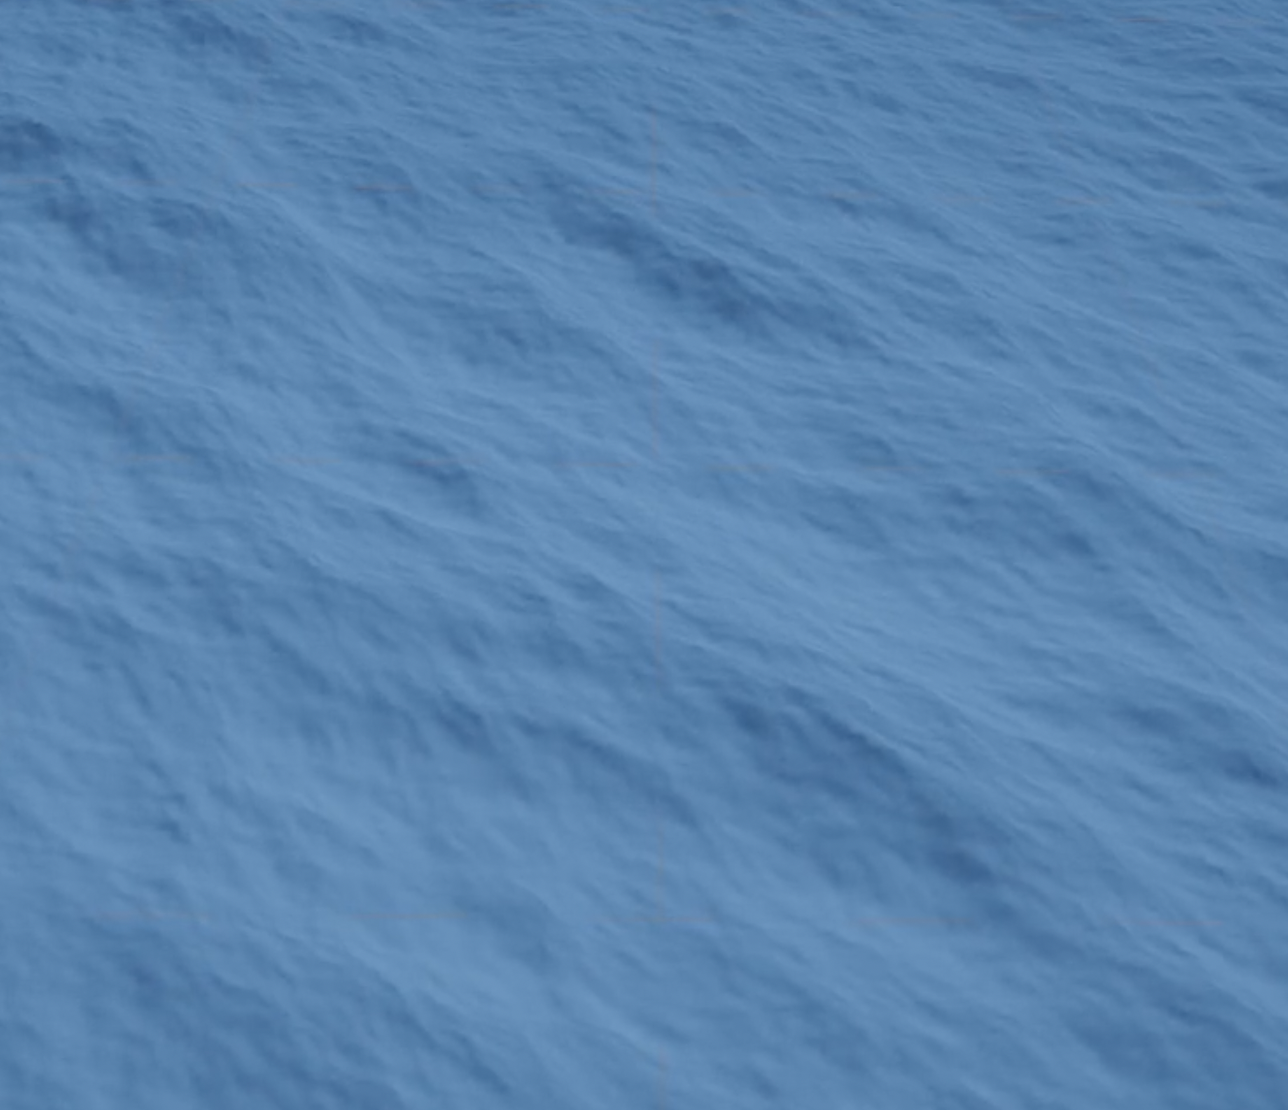
\includegraphics[width=0.8\textwidth]{"images/phillip_spectrum_comp.png"}
    \captionof{figure}{Height Map with $P_h$}
    \label{fig:phillip_spectrum_comp}
\end{minipage}
\hfill
\begin{minipage}{0.48\textwidth}
    \centering
    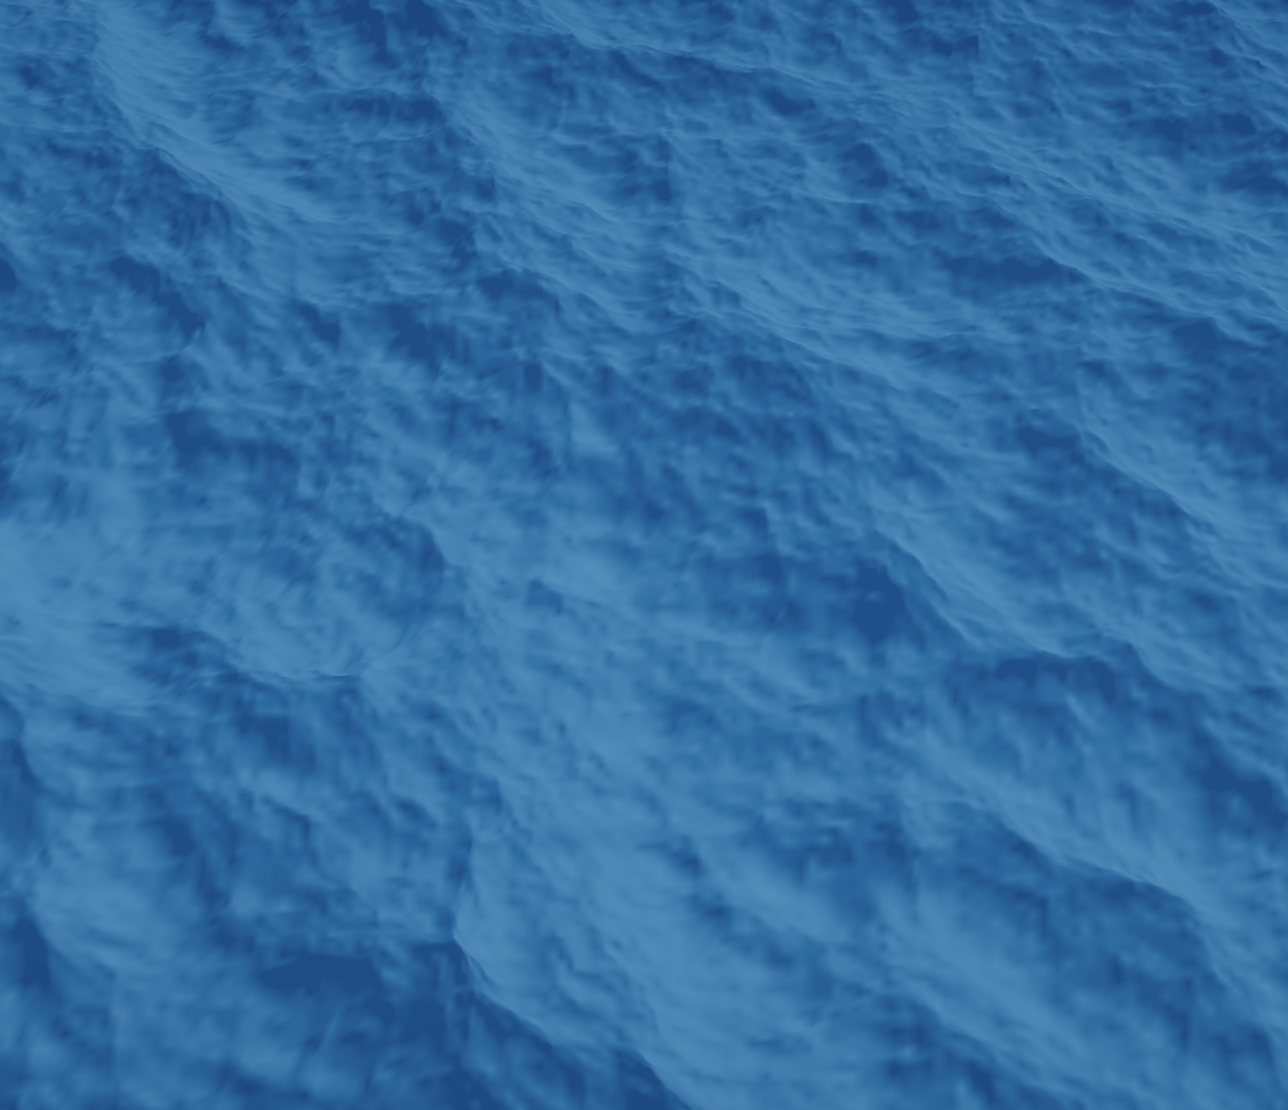
\includegraphics[width=0.8\textwidth]{"images/tma_spectrum_comp.png"}
    \captionof{figure}{Height Map using TMA Spectrum}
    \label{fig:tma_spectrum_comp}
\end{minipage}

\subsection{DFT and FFT}
The computational complexity of the DFT and FFT presents a significant contrast. With DFT operating at $O(n^2)$ and FFT at $O(n\log(n))$, the difference becomes strikingly apparent when comparing the tables \ref{tab:dft_ocean} and \ref{tab:fft_performance}. It's clear that the FFT algorithm, even when run on a lower-end M1 GPU, outperforms the DFT algorithm on a high-end Nvidia GeForce RTX 4070 GPU. For instance, the FFT on the M1 GPU for a texture size of 256x256 and 3 cascades takes 8.56ms, while the DFT on the Nvidia GPU for the same texture size but only 1 cascade takes 18.65ms. This is over twice as long, despite the Nvidia GPU being a high-end model. The difference is even more pronounced for larger texture sizes. It should be noted that the DFT was not run on the M1 GPU as it didn't have enough power to execute the algorithm.

\begin{table}[h]
    \centering
    \begin{tabular}{cccc}
        \toprule
        \textbf{GPU} & \textbf{Texture Size} & \textbf{Cascade Count} & \textbf{Time} \\
        \midrule
        \multirow{2}{*}{Nvidia GeForce RTX 4070} & 256x256 & 1 & 18.65ms \\
                                                  & 512x512 & 1 & 81.26ms \\
        \bottomrule
    \end{tabular}
    \caption{Performance of DFT}
    \label{tab:dft_ocean}
\end{table}

\subsection{Sum of Sins and FFT Based Ocean}
A comparative analysis of the visual aspects of the Sum of Sins and FFT-based approaches reveals distinct differences. The Sum of Sins approach, while capable of generating waveforms, exhibits a lack of detail that results in less realistic wave movements and energy transfers as shown in figure \ref{fig:naive_calm}. This under performance becomes dramatically apparent in stormy conditions \ref{fig:naive_stormy}, where the complexity and intensity of wave interactions are not adequately captured. However, the visual fidelity can be enhanced by integrating a pre-generated detailed water normal map, which can add complexity and depth to the visual representation.

In contrast, the FFT-based approach inherently produces more realistic results. It automatically generates highly detailed normal maps, produces choppier waves, and accurately simulates energy transfers, contributing to a more authentic representation of oceanic conditions.

\begin{minipage}{0.48\textwidth}
    \centering
    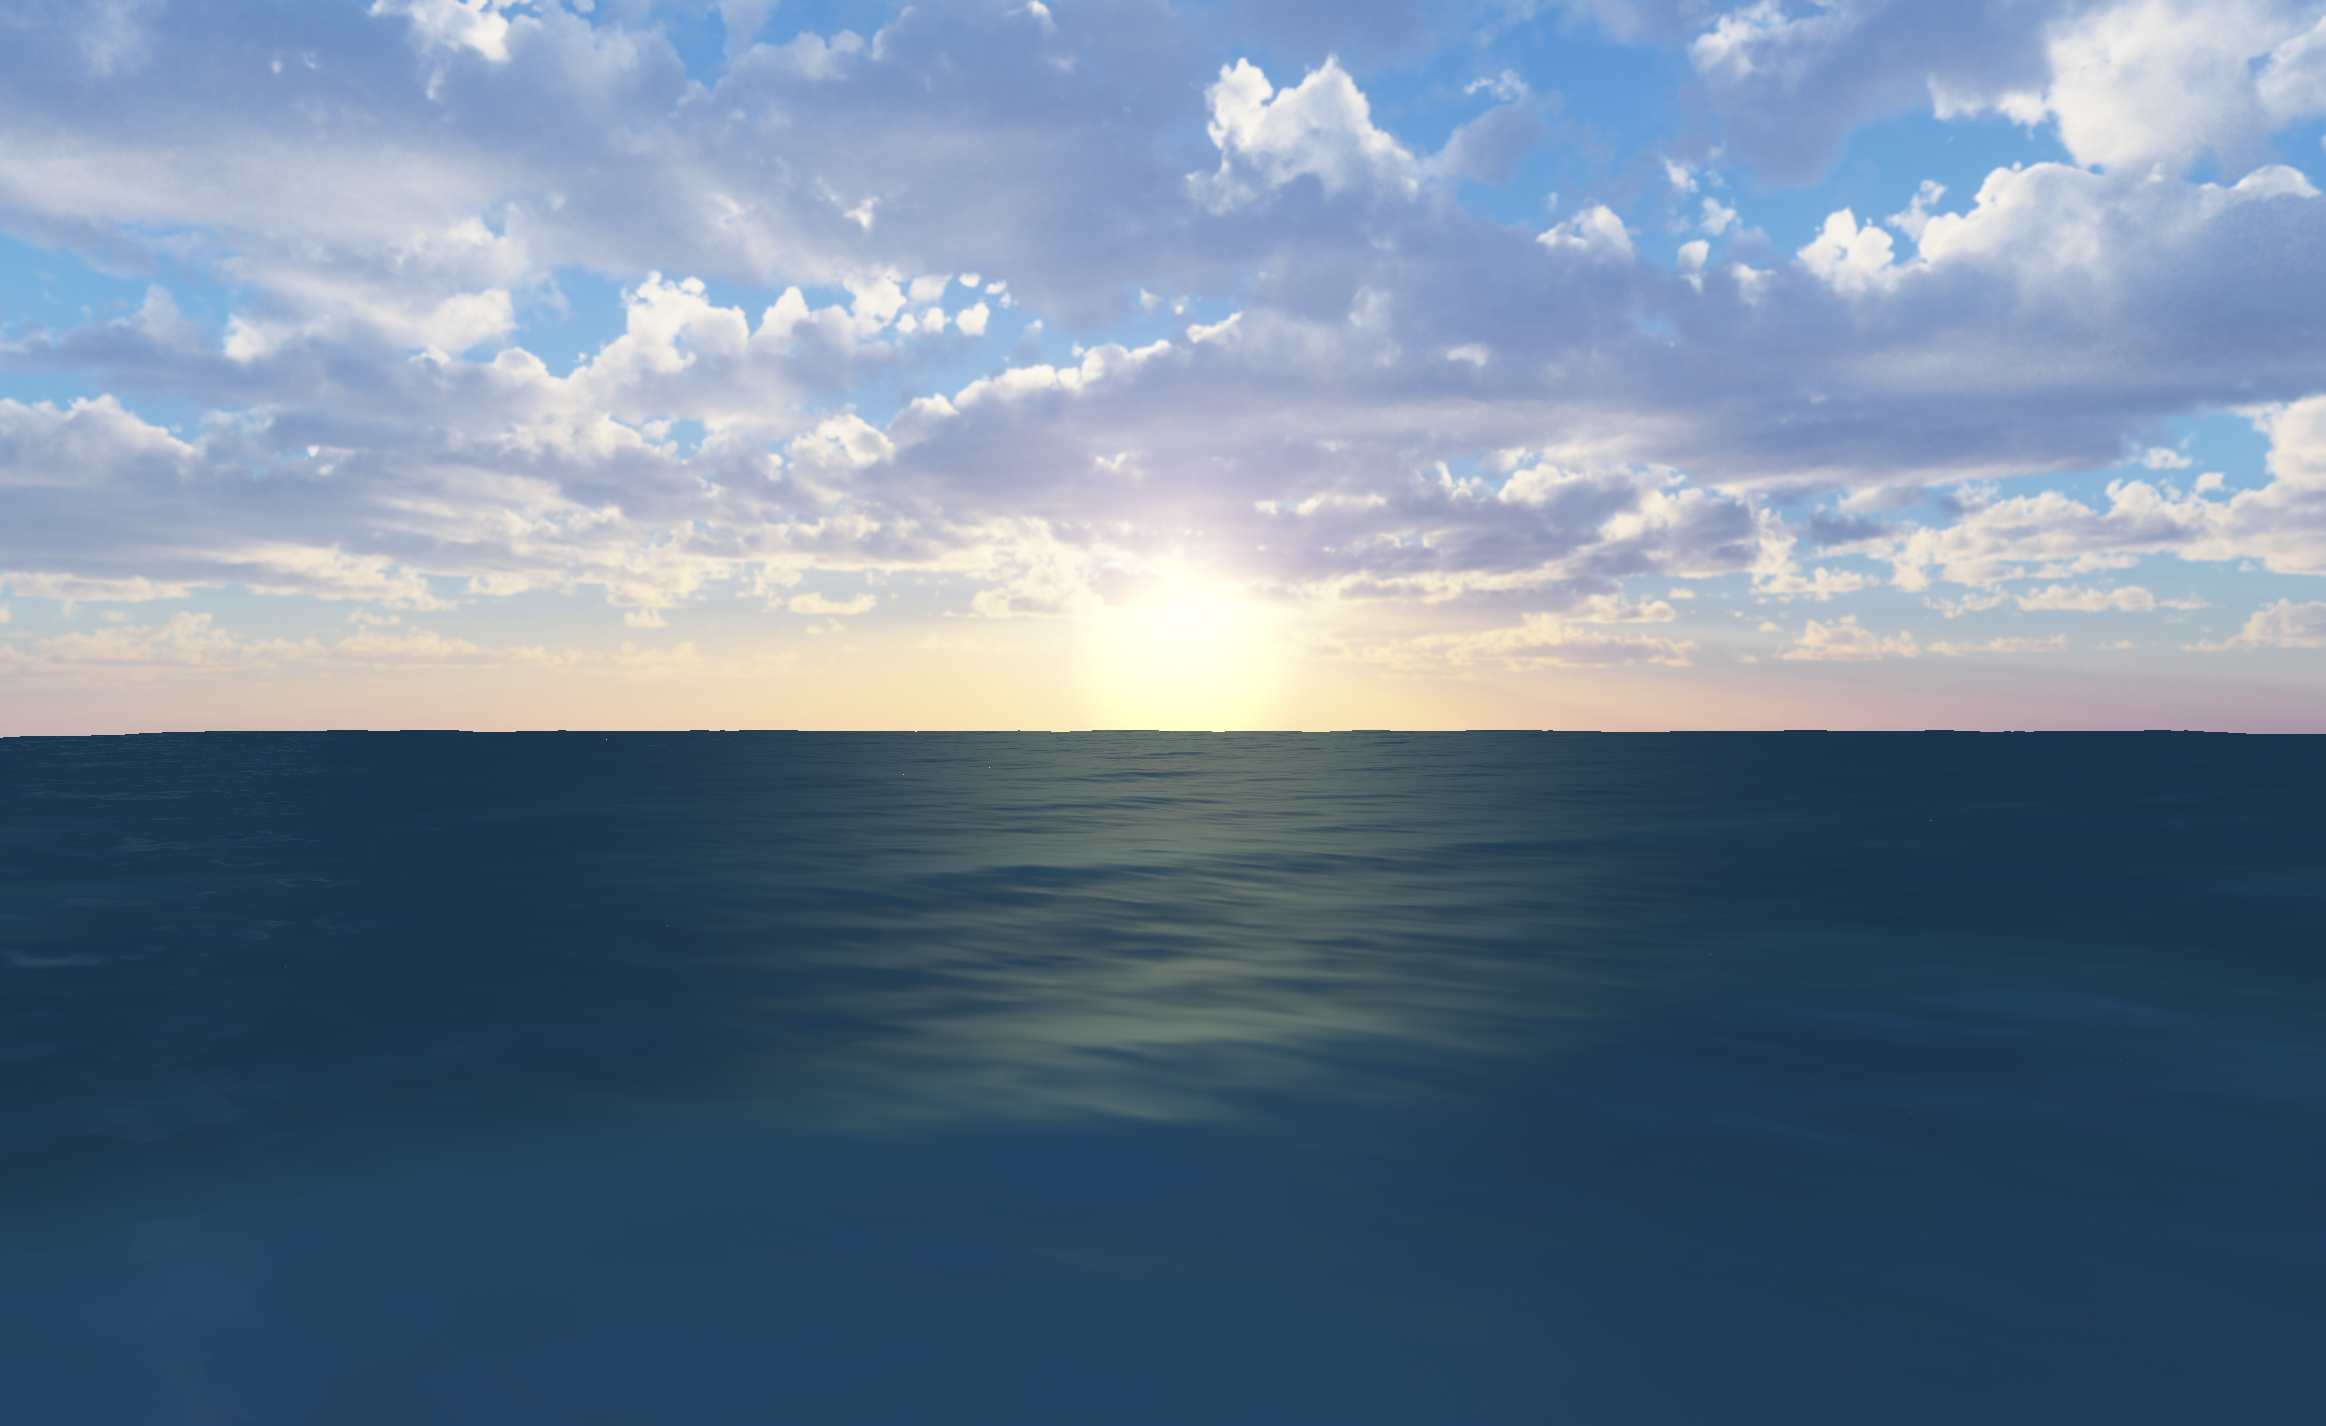
\includegraphics[width=1\textwidth]{"images/naive_calm.png"}
    \captionof{figure}{Sum Of Sines Calm Ocean}
    \label{fig:naive_calm}
\end{minipage}
\hfill
\begin{minipage}{0.48\textwidth}
    \centering
    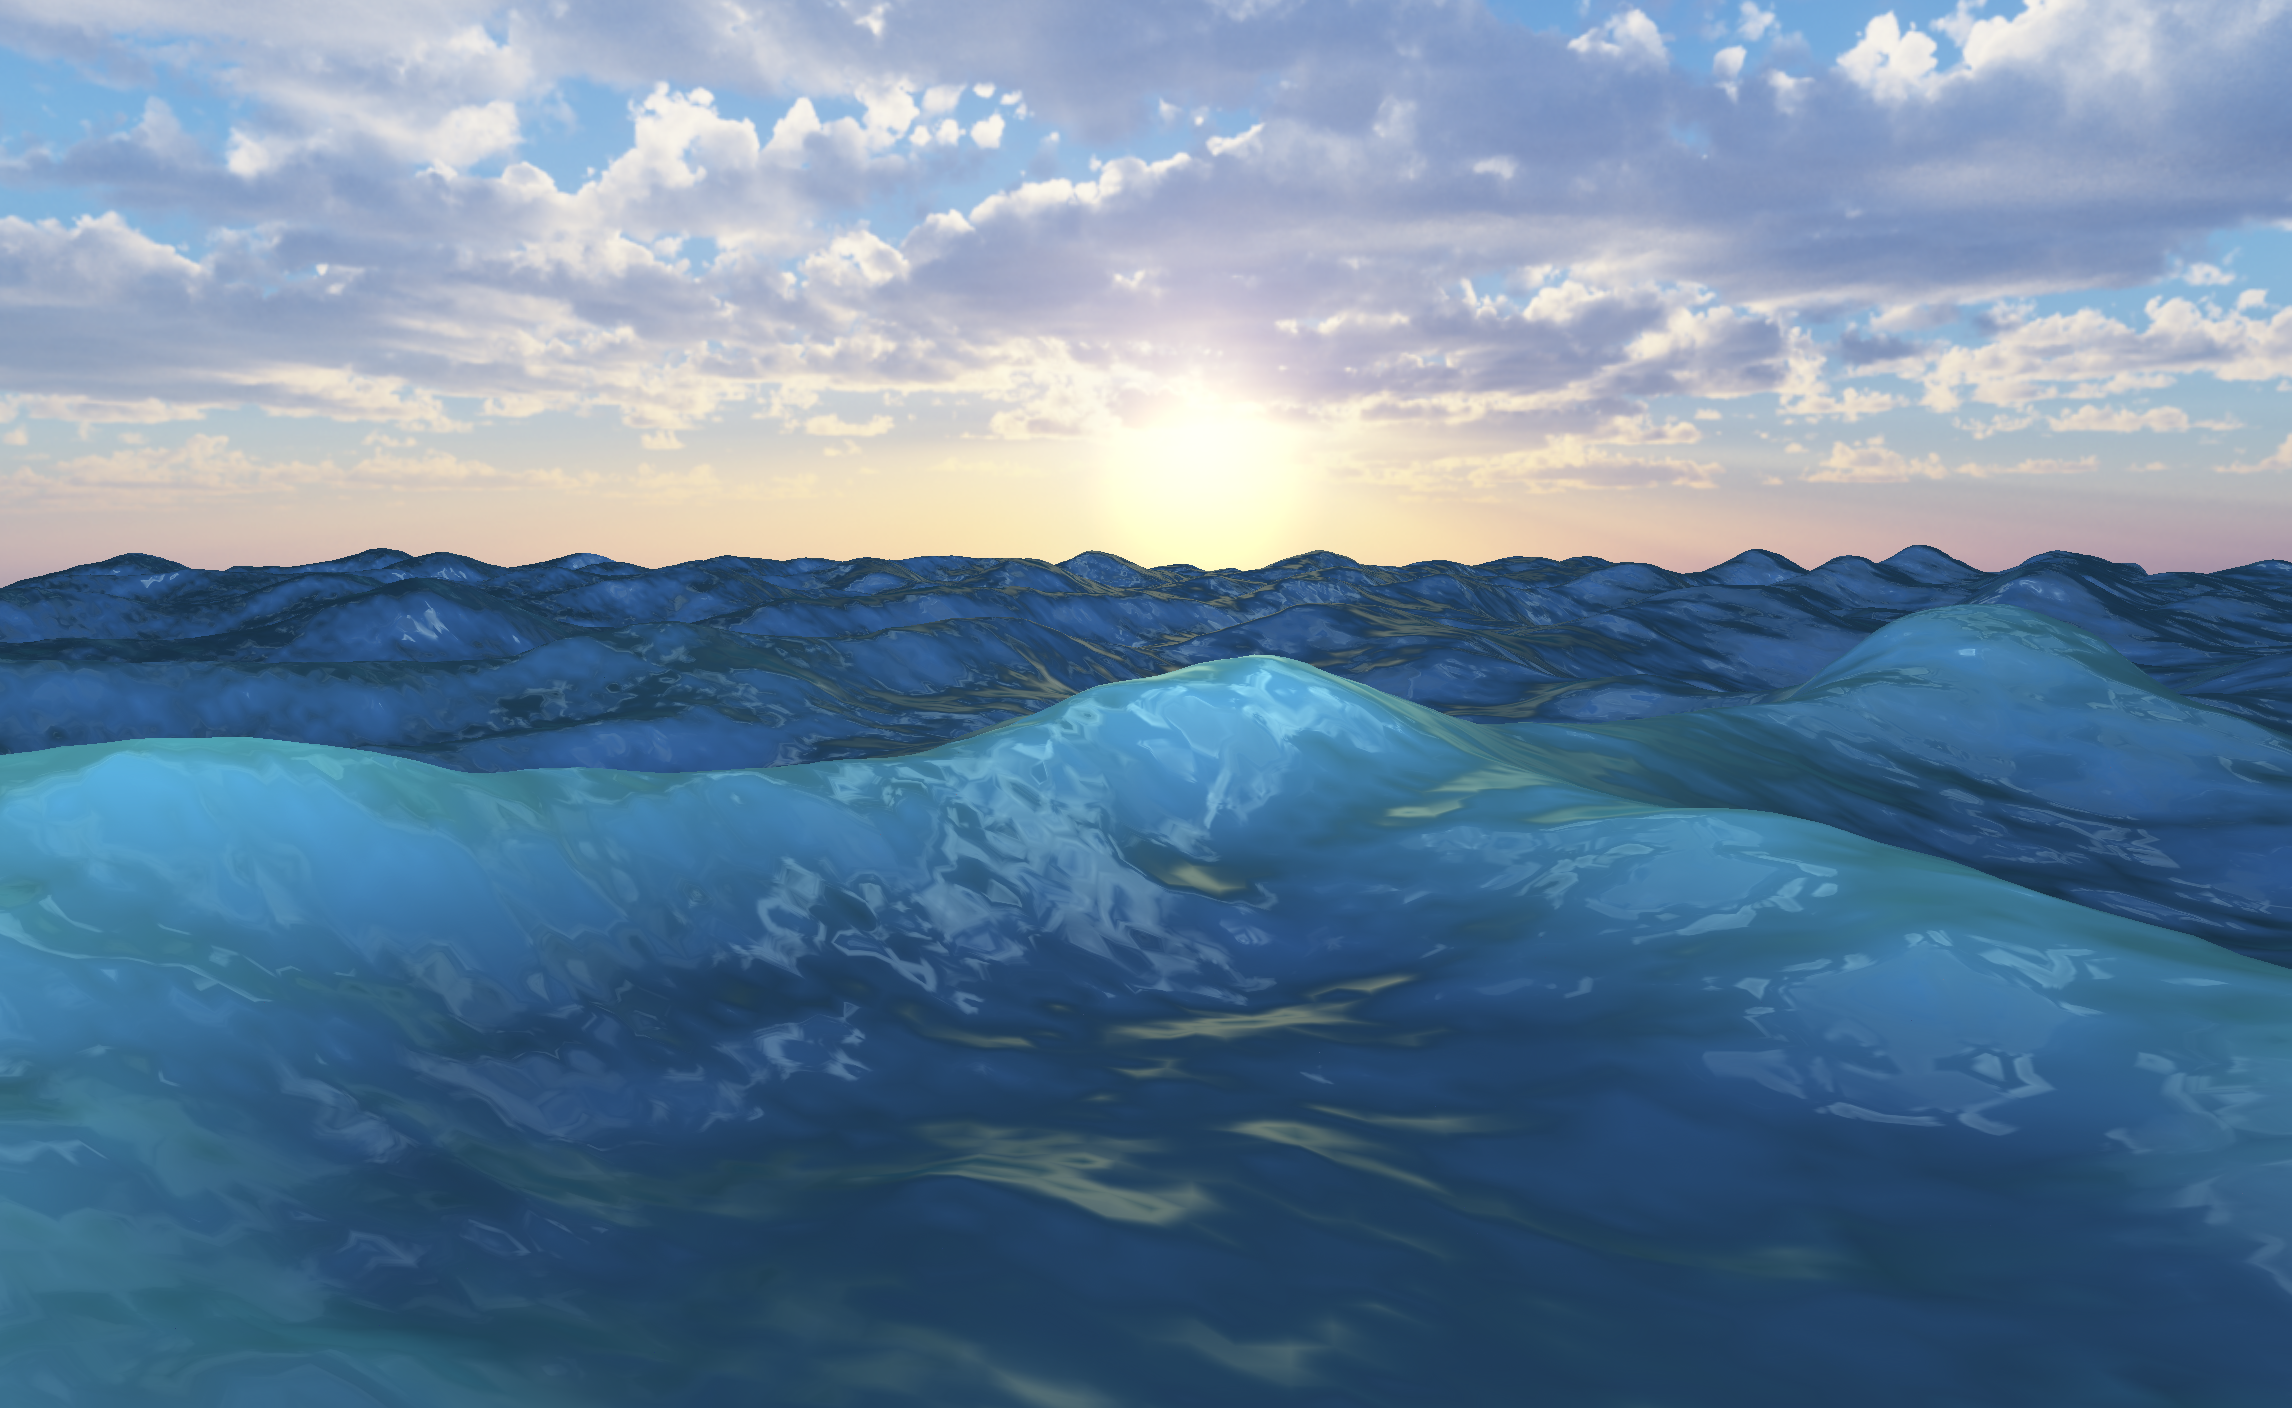
\includegraphics[width=1\textwidth]{"images/naive_storm.png"}
    \captionof{figure}{Sum Of Sines Stormy Ocean}
    \label{fig:naive_stormy}
\end{minipage}

\subsection{Real world oceans}
When it comes to calm ocean, the FFT based ocean with TMA spectrum performs extremely well and holds the desired shape as shown in figures \ref{fig:real_calm_ocean} and \ref{fig:fake_calm_ocean}.

\begin{minipage}[t]{0.48\textwidth}
    \centering
    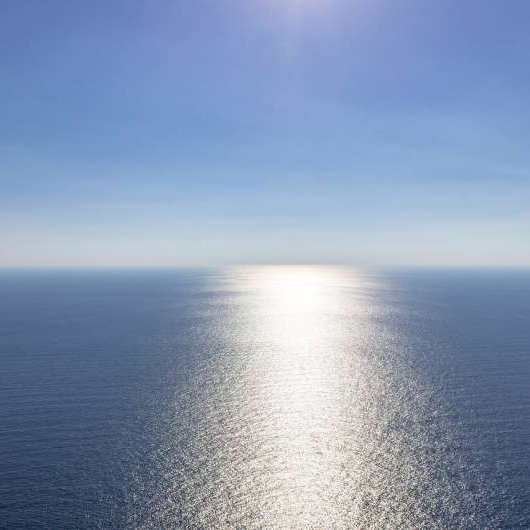
\includegraphics[width=1\textwidth]{"images/real_calm_ocean.jpg"}
    \captionsetup{justification=centering}
    \captionof{figure}{Calm Atlantic Ocean\\ Credits: CC0 Public Domain}
    \label{fig:real_calm_ocean}
\end{minipage}
\hfill
\begin{minipage}[t]{0.48\textwidth}
    \centering
    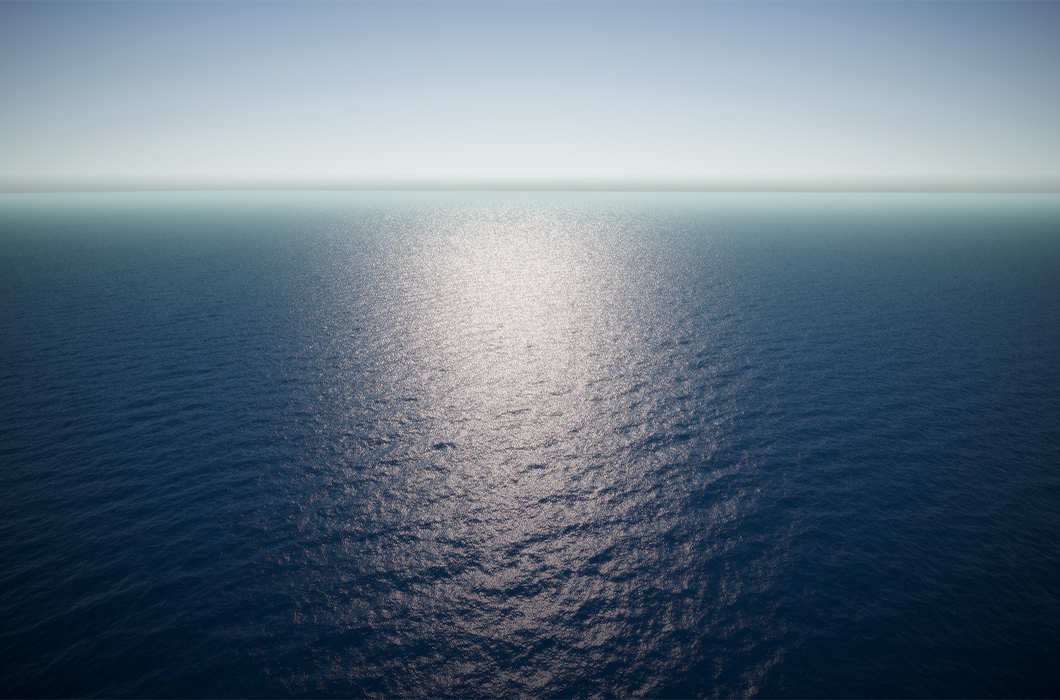
\includegraphics[width=1\textwidth]{"images/fake_calm_ocean.png"}
    \captionof{figure}{Spectrum: TMA, Size: 256x256, $l_1$: 256, $l_2$: 100, $l_3$: 10, $\lambda$: O.9, $U_{10}$: 0.5 m/s, Fetch: 1000km, Depth: 500m}
    \label{fig:fake_calm_ocean}
\end{minipage}

where each $l$ is the wave length scale of each cascade.

When it comes to stormy ocean where huge waves is expected the general shape of an ocean is still realistic
and can handle the big waves without any trouble, and because of different cascades the tilling is berley noticeable as shown in the following figures \ref{fig:real_stormy_ocean} and \ref{fig:fake_stormy_ocean}.

\begin{minipage}[t]{0.48\textwidth}
    \centering
    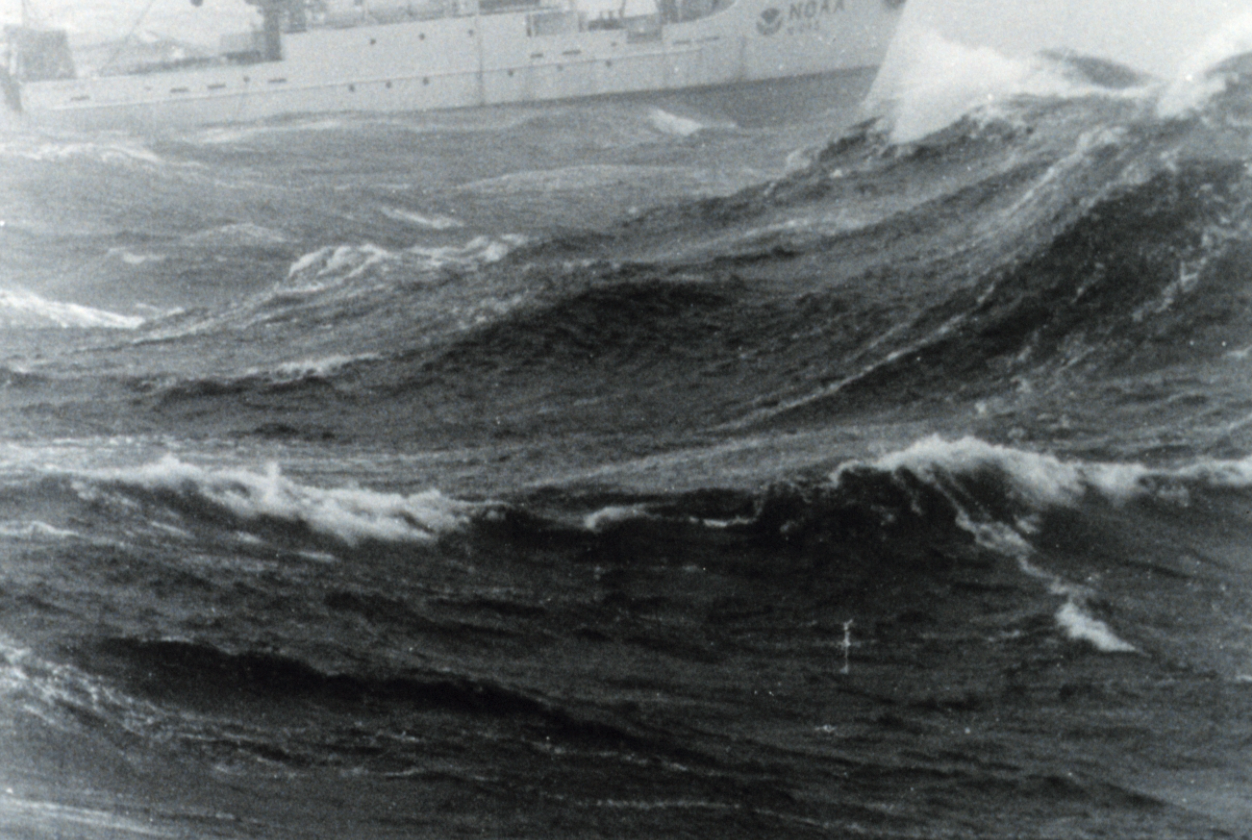
\includegraphics[width=1\textwidth]{"images/real_stormy_ocean.png"}
    \captionsetup{justification=centering}
    \captionof{figure}{Calm Atlantic Ocean\\ Credits: CC0 Public Domain}
    \label{fig:real_stormy_ocean}
\end{minipage}
\hfill
\begin{minipage}[t]{0.48\textwidth}
    \centering
    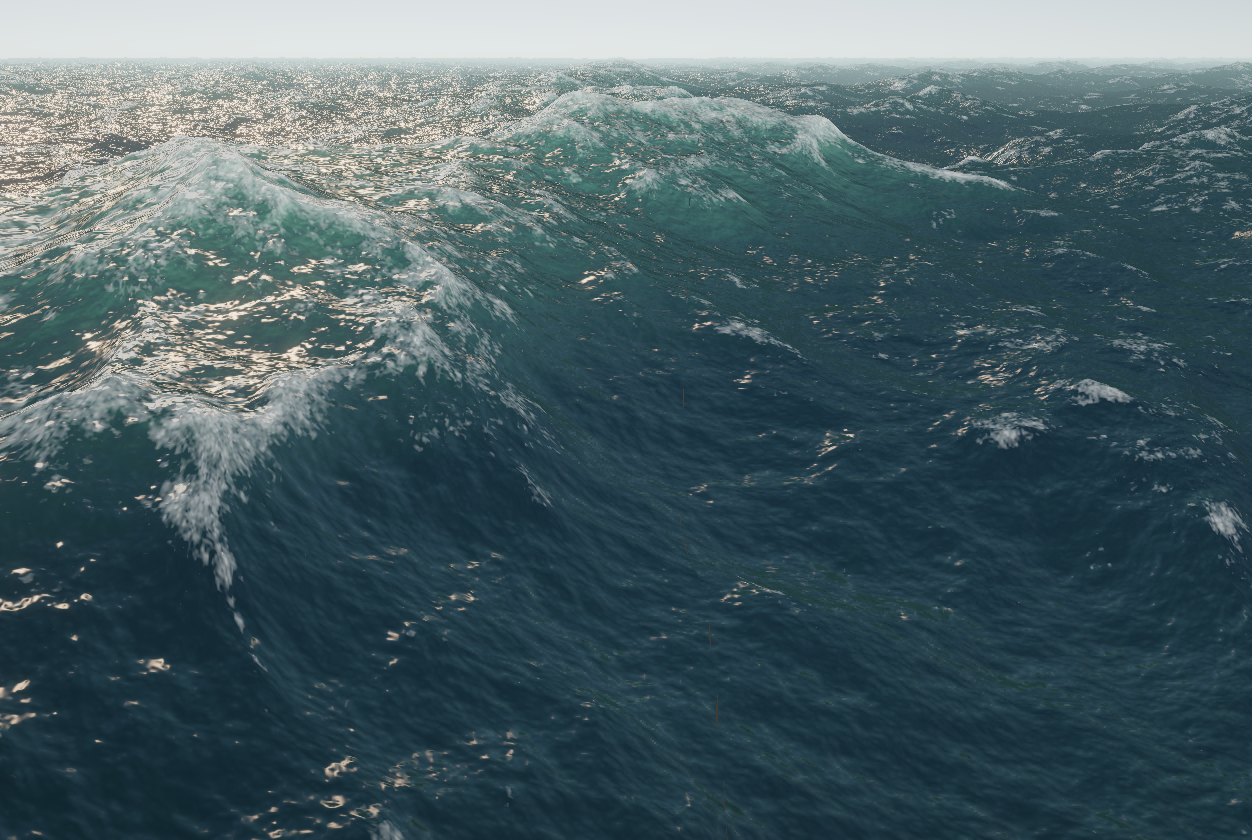
\includegraphics[width=1\textwidth]{"images/fake_stormy_ocean.png"}
    \captionof{figure}{Spectrum: TMA, Size: 256x256, $l_1$: 700, $l_2$: 256, $l_3$: 70, $\lambda$: O.9, $U_{10}$: 21 m/s, Fetch: 1000km, Depth: 500m}
    \label{fig:fake_stormy_ocean}
\end{minipage}

\subsubsection{Diffrent Outputs}
Following figures \ref{fig:output_1}, \ref{fig:output_2} and \ref{fig:output_3} are oceans with different parameters.

\begin{minipage}[t]{1\textwidth}
    \centering
    \includegraphics[width=0.75\textwidth]{"images/output1.png"}
    \captionof{figure}{Spectrum: TMA, Size: 256x256, $l_1$: 400, $l_2$: 100, $l_3$: 10, $\lambda$: O.9, $U_{10}$: 0.5 m/s, Fetch: 1000km, Depth: 500m}
    \label{fig:output_1}
\end{minipage}
\begin{minipage}[t]{1\textwidth}
    \centering
    \includegraphics[width=0.75\textwidth]{"images/output2.png"}
    \captionof{figure}{Spectrum: TMA, Size: 256x256, $l_1$: 800, $l_2$: 256, $l_3$: 10, $\lambda$: O.95, $U_{10}$: 31 m/s, Fetch: 1000km, Depth: 500m}
    \label{fig:output_2}
\end{minipage}

\begin{minipage}{1\textwidth}
    \centering
    \includegraphics[width=0.75\textwidth]{"images/output3.png"}
    \captionof{figure}{Spectrum: TMA, Size: 256x256, $l_1$: 600, $l_2$: 256, $l_3$: 10, $\lambda$: 1.3, $U_{10}$: 12 m/s, Fetch: 1000km, Depth: 500m}
    \label{fig:output_3}
\end{minipage}

\section{Limitations}
During the implementation of our FFT-based ocean generation technique, we encountered challenges related to the global application of FFT-generated maps. This global application restricts us from selectively altering specific sections of the sea, such as the wake created by a moving ship or the reduced wave height near a shallow beach.

To address these challenges, J. Tessendorf proposed a hybrid approach in his paper "iWaves" (2004) \cite{tessendorf2004}. This approach combines grid-based ocean generation, where each vertex point is propagated individually and FFT waves serve as ambient waves. Tessendorf later enhanced this approach with the release of “eWaves” \cite{tessendorf2014}.

These challenges underscore the complexities involved in ocean wave simulation and the potential of hybrid approaches in advancing the field. The proposed hybrid approach effectively addresses the identified challenges, demonstrating its potential in enhancing the realism and interactivity of ocean wave simulations.